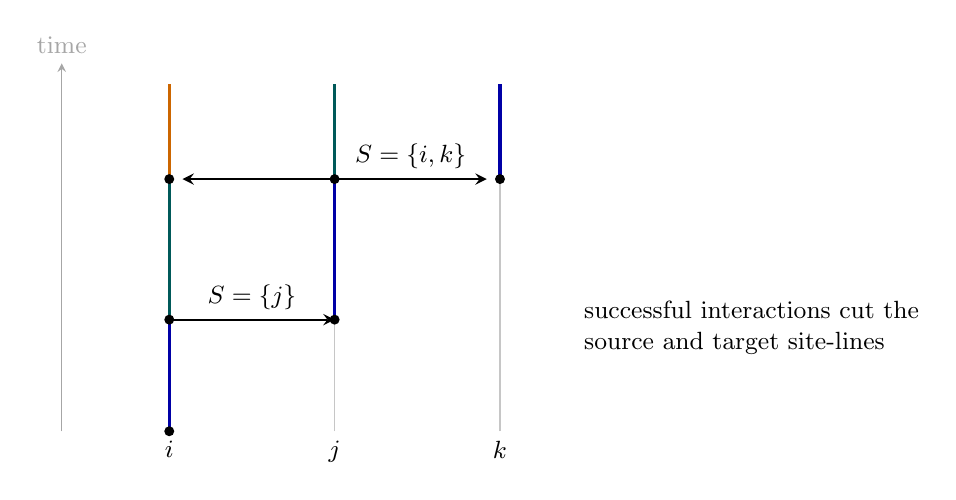
\begin{tikzpicture}[
  x=2.1cm,
  y=1.05cm,
  >=stealth,
  every node/.style={font=\small}
]
  \draw[->,gray!70] (-0.65,0) -- (-0.65,4.45) node[above] {time};

  \foreach \x/\lab in {0/\(i\),1/\(j\),2/\(k\)} {
    \draw[gray!45] (\x,0) -- (\x,4.2);
    \node[below] at (\x,0) {\lab};
  }

  \draw[very thick,blue!65!black] (0,0) -- (0,1.35);
  \draw[very thick,teal!70!black] (0,1.35) -- (0,3.05);
  \draw[very thick,orange!80!black] (0,3.05) -- (0,4.2);

  \draw[very thick,blue!65!black] (1,1.35) -- (1,3.05);
  \draw[very thick,teal!70!black] (1,3.05) -- (1,4.2);

  \draw[very thick,blue!65!black] (2,3.05) -- (2,4.2);

  \fill (0,0) circle (1.8pt);
  \fill (0,1.35) circle (1.8pt);
  \fill (1,1.35) circle (1.8pt);
  \fill (0,3.05) circle (1.8pt);
  \fill (1,3.05) circle (1.8pt);
  \fill (2,3.05) circle (1.8pt);

  \draw[->,thick] (0,1.35) -- (1,1.35)
    node[midway,above] {\(S=\{j\}\)};
  \draw[->,thick] (1,3.05) -- (0.08,3.05);
  \draw[->,thick] (1,3.05) -- (1.92,3.05)
    node[midway,above] {\(S=\{i,k\}\)};

  \node[left] at (-0.05,0.65) {\(\sI\sO\)};
  \node[left] at (-0.05,2.15) {\(\sO\sI\)};
  \node[right] at (1.05,2.15) {\(\sI\sO\)};
  \node[left] at (-0.05,3.65) {\(\sI\sE\)};
  \node[right] at (1.05,3.65) {\(\sO\sE\)};
  \node[right] at (2.05,3.65) {\(\sI\sE\)};

  \node[align=left,anchor=west] at (2.45,1.25)
    {successful interactions cut the\\source and target site-lines};
\end{tikzpicture}
